\documentclass{article}\usepackage[]{graphicx}\usepackage[]{xcolor}
% maxwidth is the original width if it is less than linewidth
% otherwise use linewidth (to make sure the graphics do not exceed the margin)
\makeatletter
\def\maxwidth{ %
  \ifdim\Gin@nat@width>\linewidth
    \linewidth
  \else
    \Gin@nat@width
  \fi
}
\makeatother

\definecolor{fgcolor}{rgb}{0.345, 0.345, 0.345}
\newcommand{\hlnum}[1]{\textcolor[rgb]{0.686,0.059,0.569}{#1}}%
\newcommand{\hlsng}[1]{\textcolor[rgb]{0.192,0.494,0.8}{#1}}%
\newcommand{\hlcom}[1]{\textcolor[rgb]{0.678,0.584,0.686}{\textit{#1}}}%
\newcommand{\hlopt}[1]{\textcolor[rgb]{0,0,0}{#1}}%
\newcommand{\hldef}[1]{\textcolor[rgb]{0.345,0.345,0.345}{#1}}%
\newcommand{\hlkwa}[1]{\textcolor[rgb]{0.161,0.373,0.58}{\textbf{#1}}}%
\newcommand{\hlkwb}[1]{\textcolor[rgb]{0.69,0.353,0.396}{#1}}%
\newcommand{\hlkwc}[1]{\textcolor[rgb]{0.333,0.667,0.333}{#1}}%
\newcommand{\hlkwd}[1]{\textcolor[rgb]{0.737,0.353,0.396}{\textbf{#1}}}%
\let\hlipl\hlkwb

\usepackage{framed}
\makeatletter
\newenvironment{kframe}{%
 \def\at@end@of@kframe{}%
 \ifinner\ifhmode%
  \def\at@end@of@kframe{\end{minipage}}%
  \begin{minipage}{\columnwidth}%
 \fi\fi%
 \def\FrameCommand##1{\hskip\@totalleftmargin \hskip-\fboxsep
 \colorbox{shadecolor}{##1}\hskip-\fboxsep
     % There is no \\@totalrightmargin, so:
     \hskip-\linewidth \hskip-\@totalleftmargin \hskip\columnwidth}%
 \MakeFramed {\advance\hsize-\width
   \@totalleftmargin\z@ \linewidth\hsize
   \@setminipage}}%
 {\par\unskip\endMakeFramed%
 \at@end@of@kframe}
\makeatother

\definecolor{shadecolor}{rgb}{.97, .97, .97}
\definecolor{messagecolor}{rgb}{0, 0, 0}
\definecolor{warningcolor}{rgb}{1, 0, 1}
\definecolor{errorcolor}{rgb}{1, 0, 0}
\newenvironment{knitrout}{}{} % an empty environment to be redefined in TeX

\usepackage{alltt}
\usepackage{amsmath} %This allows me to use the align functionality.
                     %If you find yourself trying to replicate
                     %something you found online, ensure you're
                     %loading the necessary packages!
\usepackage{amsfonts}%Math font
\usepackage{graphicx}%For including graphics
\usepackage{hyperref}%For Hyperlinks
\usepackage[shortlabels]{enumitem}% For enumerated lists with labels specified
                                  % We had to run tlmgr_install("enumitem") in R
\hypersetup{colorlinks = true,citecolor=black} %set citations to have black (not green) color
\usepackage{natbib}        %For the bibliography
\setlength{\bibsep}{0pt plus 0.3ex}
\bibliographystyle{apalike}%For the bibliography
\usepackage[margin=0.50in]{geometry}
\usepackage{float}
\usepackage{multicol}

%fix for figures
\usepackage{caption}
\newenvironment{Figure}
  {\par\medskip\noindent\minipage{\linewidth}}
  {\endminipage\par\medskip}
\IfFileExists{upquote.sty}{\usepackage{upquote}}{}
\begin{document}

\vspace{-1in}
\title{Lab 7+8 -- MATH 240 -- Computational Statistics}

\author{
  Henry Sun \\
  Colgate University  \\
  Mathematics  \\
  {\tt }
}

\date{04/01/2025}

\maketitle

\begin{multicols}{2}
\begin{abstract}
This document provides a basic template for the 2-page labs we will complete each week. Here, briefly summarize what you did and why it might be helpful. Provide all the top-line conclusions, but avoid providing \emph{all} the details. Results should be limited to ``we show X, Y, and Z."
\end{abstract}

\noindent \textbf{Keywords:} What topics does the lab cover concerning class? List 3-4 key terms here, separated by semicolons.

\section{Introduction}
In this lab, we explored the beta distribution in great detail. The beta distribution is a continuous distribution, modeling the
Provide an overarching summary of what you're talking about. In this section, you introduce the idea to the reader, and your goal is to pull them in. What's the mystery you aim to solve?

You want to provide enough background to understand the context of the work. Specifically, what is the question you are addressing? If it applies, describe what information currently exists about this problem, including citations, and explain how the question you're answering complements this work.

Provide a roadmap of the structure of the paper. 

\section{Density Functions and Parameters}
As the beta distribution is a continuous distribution, it has a probability density function (PDF) and a cumulative density function (CDF). It takes two shape parameters, $\alpha$ and $\beta$, which are both positive numbers. In \texttt{R}, the parameters for $\alpha$ and $\beta$ are \texttt{shape1} and \texttt{shape2}. The beta distribution's probability density function is given as:
 \[f_X(x|\alpha, \beta) = \frac{\Gamma(\alpha + \beta)}{\Gamma\alpha\Gamma\beta} x^{\alpha-1}(1-x)^{\beta-1}I(x \in [0,1]).\]
For the beta distribution, $I(x \in [0,1]) = 1$ when $x \in [0,1]$ and $0$ otherwise, as the support of a random variable $X$ is $[0,1]$ in the beta distribution. For some data, like the example we will look at later in the lab, data must be transformed to fit the support. 

\section{Properties and Statistics}
Various properties of the beta distribution are based on the shape parameters of the beta distribution. The beta distribution is very flexible with regards to its shape. The various statistics, such as the mean, variance, skewness, and excess kurtosis can be written in terms of $\alpha$ and $\beta$: 
 \begin{align*}
 E(X) = \frac{\alpha}{\alpha + \beta} \tag{The Mean}\\
var(X) = \frac{\alpha\beta}{(\alpha + \beta)^2(\alpha + \beta + 1)} \tag{The Variance} \\
skew(X) = \frac{2(\beta - \alpha)\sqrt{\alpha + \beta + 1}}{(\alpha + \beta + 2)\sqrt{\alpha\beta}} \tag{The Skewness}
 \end{align*}
 \[kurt(X) = \frac{6[(\alpha - \beta)^2(\alpha + \beta + 1) - \alpha\beta(\alpha + \beta + 2)]}{\alpha\beta(\alpha + \beta + 2)(\alpha + \beta + 3)}\]
\begin{flushright}
(The Excess Kurtosis)
\end{flushright}
It's key to note that in \texttt{R}, \verb|kurt()| calculates the excess kurtosis and not the kurtosis. Instead, kurtosis = excess kurtosis + 3, or \verb|kurt(X) + 3|. \\
\indent However, by computing the moments of the beta function, we write each statistic as a combination of various $k$th centered and uncentered moments. 
\begin{align*}
 \mu_X = E(X) \tag{The Mean}\\
 var(X) = \sigma^2_X = E[(X-\mu_X)]^2 \tag{The Variance}\\
 skew(X) = \frac{E[(X - \mu_X)^3]}{E[(X-\mu_X)^2]^{3/2}} \tag{The Skewness}\\
 kurt(X) = \frac{E[(X-\mu_X)^4]}{E[(X-\mu_X)^2]^2} - 3 \tag{The Excess Kurtsosis}
\end{align*}
For the beta distribution, the $k$th uncentered and centered moments are
\[E(X^{k}) = \int_{\chi}^{} x^{k}f_x(x) \,dx \]
\begin{center}
and 
\end{center}
\[E((X-\mu_X)^{k}) = \int_{\chi}^{} (x-\mu_X)^{k}f_x(x) \,dx \]
respectively. For the purposes of this lab, we wrote a function \verb|beta.moment(alpha, beta, k, centered)| to help us compute the population-level characteristics using this moments. \textbf{maybe add code snippet here} \\

Due to the beta distribution's flexiblity, it can take on numerous different shapes, can be right-skewed, platykurtic, etc. Below is a data summary of this. 
\textbf{reference a figure showing this.}

\subsection{Intro Subsection}
You might need/want to discuss the topics in subsections. Or, you may have multiple questions.

% \begin{Figure}
% \includegraphics{screenshot}
% \end{Figure}

\section{Methods}
Describe the data you are working with, if applicable. Describe the specific process you will follow to answer the question at hand. This does not mean you should write something like this.
\begin{quote}
\textit{I did this and then I did that and then I did this other thing and then..., and then..., and then...}
\end{quote}
Instead, it should provide a clear and concise narrative that flows from the problem specification in the Introduction to how you will approach answering it. This is where I would expect to see some citations for \texttt{R} packages you will use to conduct the statistical analysis reported in the Results section.


\subsection{Methods Subsection}
Much like the Introduction, subsections can be helpful for the Methods section. For example, you might describe data collection and the statistical analyses of the collected data in different subsections. Or, you may have different questions that require distinct methods. 

\section{Results}
Tie together the Introduction -- where you introduce the problem at hand -- and the methods --  what you propose to do to answer the question. Present your data, the results of your analyses, and how each reported aspect contributes to answering the question. This section should include table(s), statistic(s), and graphical displays. Make sure to put the results in a sensible order and that each result contributes a logical and developed solution. It should not just be a list. Avoid being repetitive. 

\subsection{Results Subsection}
Subsections can be helpful for the Results section, too. This can be particularly helpful if you have different questions to answer. 


\section{Discussion}
 You should objectively evaluate the evidence you found in the data. Do not embellish or wish-terpet (my made-up phase for making an interpretation you, or the researcher, wants to be true without the data \emph{actually} supporting it). Connect your findings to the existing information you provided in the Introduction.

Finally, provide some concluding remarks that tie together the entire paper. Think of the last part of the results as abstract-like. Tell the reader what they just consumed -- what's the takeaway message?

%%%%%%%%%%%%%%%%%%%%%%%%%%%%%%%%%%%%%%%%%%%%%%%%%%%%%%%%%%%%%%%%%%%%%%%%%%%%%%%%
% Bibliography
%%%%%%%%%%%%%%%%%%%%%%%%%%%%%%%%%%%%%%%%%%%%%%%%%%%%%%%%%%%%%%%%%%%%%%%%%%%%%%%%
\vspace{2em}

\noindent\textbf{Bibliography:} Note that when you add citations to your bib.bib file \emph{and}
you cite them in your document, the bibliography section will automatically populate here.

\begin{tiny}
\bibliography{bib}
\end{tiny}
\end{multicols}

%%%%%%%%%%%%%%%%%%%%%%%%%%%%%%%%%%%%%%%%%%%%%%%%%%%%%%%%%%%%%%%%%%%%%%%%%%%%%%%%
% Appendix
%%%%%%%%%%%%%%%%%%%%%%%%%%%%%%%%%%%%%%%%%%%%%%%%%%%%%%%%%%%%%%%%%%%%%%%%%%%%%%%%
\newpage
\onecolumn
\section{Appendix}
 \begin{figure}[H]
 \begin{center}
\begin{knitrout}
\definecolor{shadecolor}{rgb}{0.969, 0.969, 0.969}\color{fgcolor}
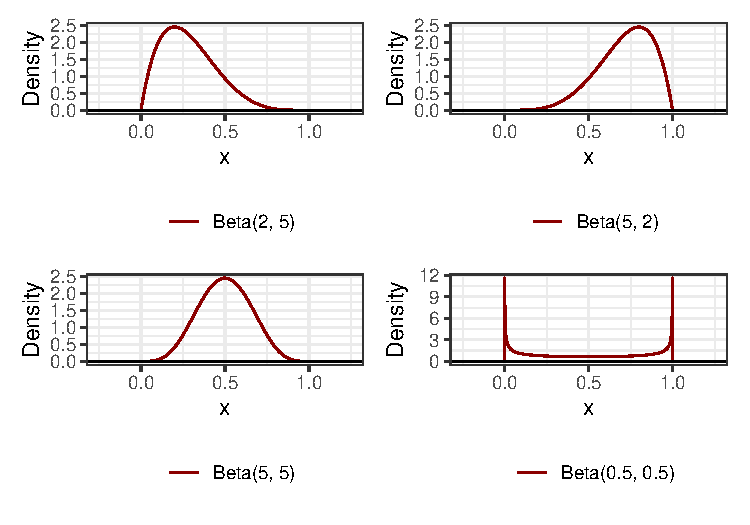
\includegraphics[width=\maxwidth]{figure/unnamed-chunk-2-1} 
\end{knitrout}
 \caption{Plotting of various different beta PDFs.}
 \label{plot1} %we can now reference plot1
 \end{center}
 \end{figure}
 \begin{table}[ht]
\centering
\begin{tabular}{rrrrrrr}
  \hline
  alpha & beta & mean & variance & skewness & e.kurtosis \\ 
  \hline
  2.00 & 5.00 & 0.29 & 0.03 & 0.60 & -0.12 \\ 
  5.00 & 5.00 & 0.50 & 0.02 & 0.00 & -0.46 \\ 
  5.00 & 2.00 & 0.71 & 0.03 & -0.60 & -0.12 \\ 
  0.50 & 0.50 & 0.50 & 0.12 & 0.00 & -1.50 \\ 
   \hline
\end{tabular}
\caption{task 1 table}
\label{table1}
\end{table}

\begin{table}[ht]
\centering
\begin{tabular}{rrrrrrr}
  \hline
  alpha & beta & mean & variance & skewness & e.kurtosis \\ 
  \hline
  2.00 & 5.00 & 0.29 & 0.03 & 0.57 & -0.22 \\ 
  5.00 & 5.00 & 0.50 & 0.02 & -0.06 & -0.57 \\ 
  5.00 & 2.00 & 0.71 & 0.03 & -0.57 & -0.22 \\ 
  0.50 & 0.50 & 0.51 & 0.13 & -0.02 & -1.50 \\ 
   \hline
\end{tabular}
\caption{task 3 table}
\label{table2}
\end{table}

\begin{figure}[H]
 \begin{center}
\begin{knitrout}
\definecolor{shadecolor}{rgb}{0.969, 0.969, 0.969}\color{fgcolor}
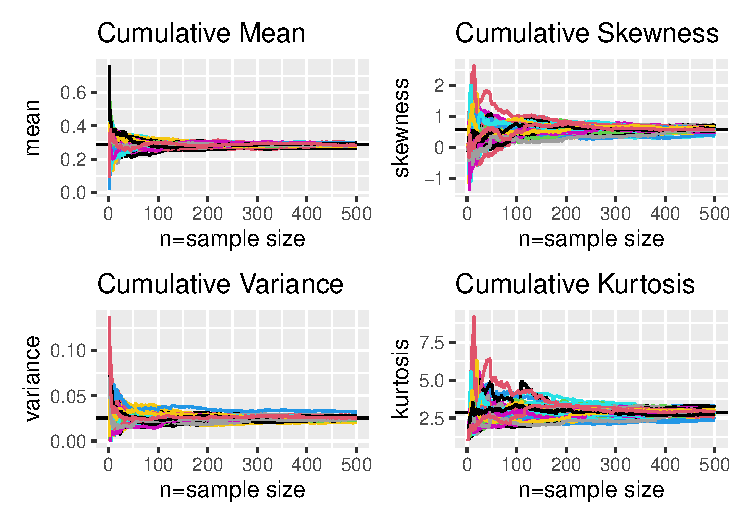
\includegraphics[width=\maxwidth]{figure/unnamed-chunk-3-1} 
\end{knitrout}
 \caption{task 3 histograms}
 \label{plot2} %we can now reference plot1
 \end{center}
 \end{figure}

\begin{figure}[H]
 \begin{center}
\begin{knitrout}
\definecolor{shadecolor}{rgb}{0.969, 0.969, 0.969}\color{fgcolor}
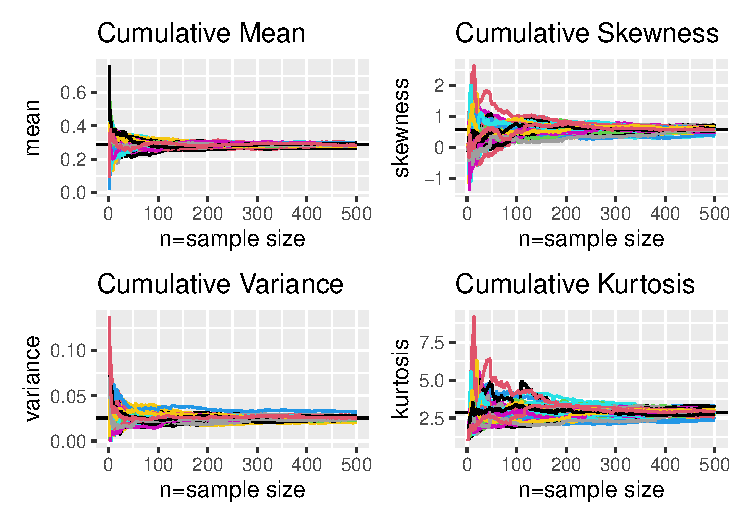
\includegraphics[width=\maxwidth]{figure/unnamed-chunk-4-1} 
\end{knitrout}
 \caption{cumstats plots}
 \label{plot3} %we can now reference plot1
 \end{center}
 \end{figure}

\begin{figure}[H]
 \begin{center}
\begin{knitrout}
\definecolor{shadecolor}{rgb}{0.969, 0.969, 0.969}\color{fgcolor}
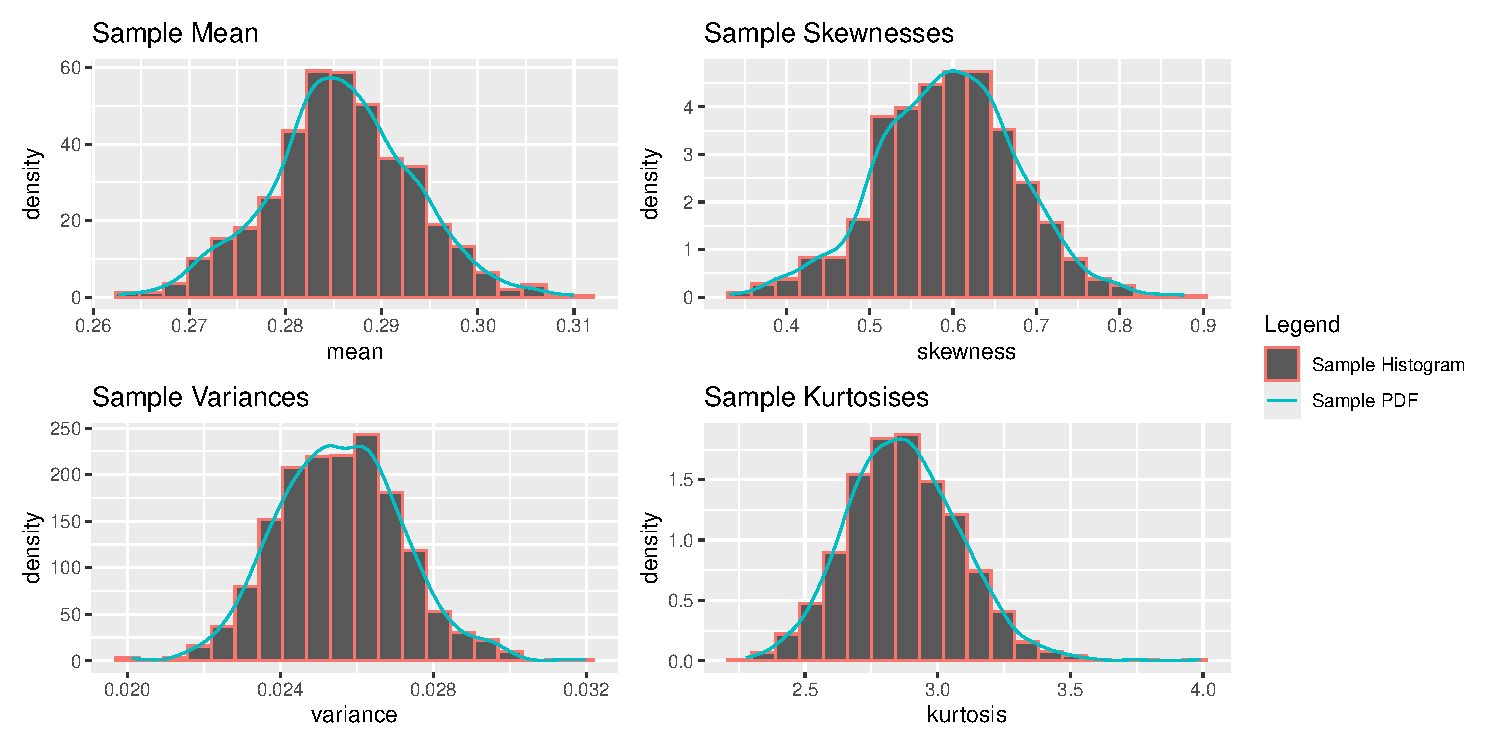
\includegraphics[width=\maxwidth]{figure/unnamed-chunk-5-1} 
\end{knitrout}
 \caption{stats samplings dist plots}
 \label{plot4} %we can now reference plot1
 \end{center}
 \end{figure}
 
 \begin{table}[ht]
\centering
\begin{tabular}{rllrrr}
  \hline
 parameters & method & bias & precision & mse \\ 
  \hline
    Alpha & MOM & 0.08 & 1.83 & 0.63 \\ 
    Alpha & MLE & 0.07 & 2.13 & 0.54 \\ 
    Beta & MOM & 10.29 & 0.00 & 8192.93 \\ 
    Beta & MLE & 9.11 & 0.00 & 7058.82 \\ 
   \hline
\end{tabular}
\caption{mles moms}
\label{table3}

\begin{figure}[H]
 \begin{center}
\begin{knitrout}
\definecolor{shadecolor}{rgb}{0.969, 0.969, 0.969}\color{fgcolor}
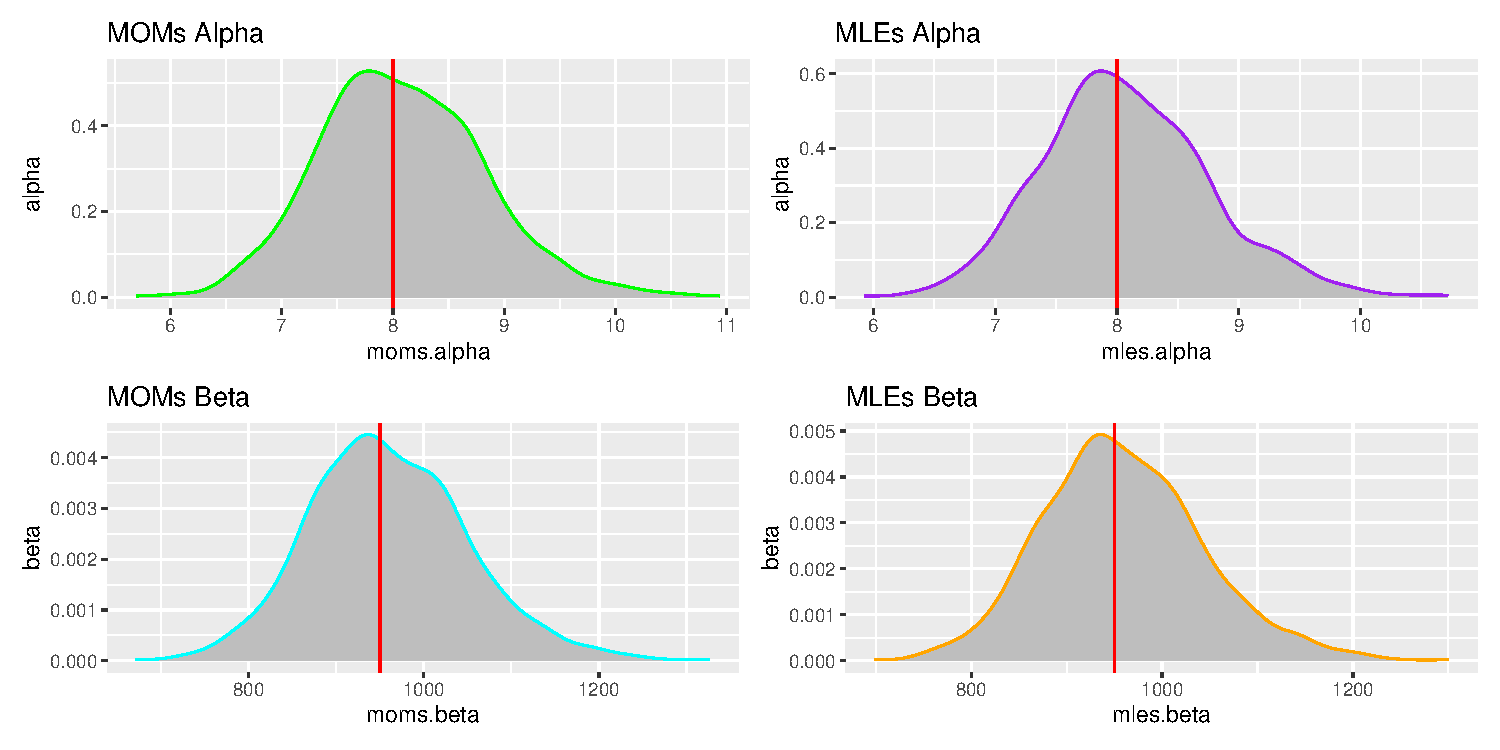
\includegraphics[width=\maxwidth]{figure/unnamed-chunk-6-1} 
\end{knitrout}
 \caption{moms mles}
 \label{plot5} %we can now reference plot1
 \end{center}
 \end{figure}

\end{table}
\end{document}
